% Ubah judul dan label berikut sesuai dengan yang diinginkan.
\section{Metodologi}
\label{sec:arsitektur}

% Ubah paragraf-paragraf pada bagian ini sesuai dengan yang diinginkan.

Metodologi yang digunakan dalam pengerjaan Tugas Akhir ini adalah sebagai berikut.
\begin{figure} [ht]
  \centering
  % Ubah sesuai dengan nama file gambar dan ukuran yang akan digunakan.
  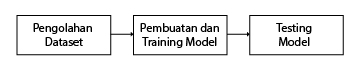
\includegraphics[width=0.5\textwidth]{gambar/metodologi.jpg}

  % Ubah sesuai dengan keterangan gambar yang diinginkan.
  \caption{Diagram blok metodologi.}
  \label{fig:metodologi}
\end{figure}


Pada tahap awal, dataset yang digunakan akan dicek dan dibagi berdasarkan training, validation dan 
testing, serta menyiapkan dataset untuk digunakan pada pembuatan model nantinya. Kemudian 
memilih model atau arsitektur Convolutional Neural Network atau CNN yang tepat sesuai dengan UTKFace 
dataset yang telah disediakan sebelumnya dan membangun model untuk keperluan training.
Di tahap training, dataset akan digunakan untuk melatih komputer dengan cara mengolah gambar dan anotasi 
yang telah dibuat sehingga terbentuk pola atau karakteristik dari masing masing kelas yang akan 
menjadi bahan pertimbangan komputer dalam mencapai sebuah keputusan atau melakukan prediksi. 
Proses training akan dilakukan menggunakan Covolutional Neural Network atau CNN pada citra wajah 
yang diberikan. Model yang sudah jadi akan dievaluasi dan dilakukan testing dengan dataset
yang telah disediakan. Untuk meningkatkan akurasi, akan dilakukan pengaturan untuk 
meningkatkan peforma dan keakuratan model.


\subsection{Pengolahan Dataset}
\label{subsec:pengolahandataset}

Pada cetak biru yang tertera pada Gambar \ref{fig:pengolahandataset}. \lipsum[8]

% Contoh input gambar pada kolom.
\begin{figure} [ht]
  \centering
  % Ubah sesuai dengan nama file gambar dan ukuran yang akan digunakan.
  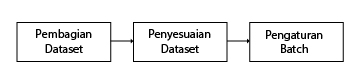
\includegraphics[width=0.5\textwidth]{gambar/dataset.jpg}

  % Ubah sesuai dengan keterangan gambar yang diinginkan.
  \caption{Urutan Pengolahan Dataset}
  \label{fig:pengolahandataset}
\end{figure}

\lipsum[9-10]

\subsection{Pembuatan dan Training Model}
\label{subsec:model}

\lipsum[11]

\begin{figure} [ht]
  \centering
  % Ubah sesuai dengan nama file gambar dan ukuran yang akan digunakan.
  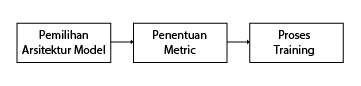
\includegraphics[width=0.5\textwidth]{gambar/model.jpg}

  % Ubah sesuai dengan keterangan gambar yang diinginkan.
  \caption{Urutan Pembuatan Dataset}
  \label{fig:model}
\end{figure}

% Contoh pembuatan potongan kode.
\begin{lstlisting}[
  language=C++,
  caption={Program halo dunia.},
  label={lst:halodunia}
]
#include <iostream>

int main() {
    std::cout << "Halo Dunia!";
    return 0;
}
\end{lstlisting}

\lipsum[12]

% Contoh pembuatan daftar.
\begin{enumerate}
  \item \lipsum[13][1-4]
  \item \lipsum[13][5-8]
  \item \lipsum[13][9-12]
\end{enumerate}

\lipsum[14-15]

\subsection{Testing Model}
\label{subsec:testing}

\lipsum[11]

\begin{figure} [ht]
  \centering
  % Ubah sesuai dengan nama file gambar dan ukuran yang akan digunakan.
  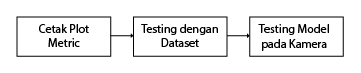
\includegraphics[width=0.5\textwidth]{gambar/testing.jpg}

  % Ubah sesuai dengan keterangan gambar yang diinginkan.
  \caption{Urutan Testing Model}
  \label{fig:testing}
\end{figure}
